\documentclass{ctexart}
\usepackage{graphicx}
\usepackage{caption}
\usepackage{float}
\usepackage{amsmath}
\usepackage{fancyhdr}
\usepackage{xunicode-addon}
\usepackage{booktabs}
\usepackage{listings}
\usepackage{hyperref}
\usepackage[a4paper,hmargin=1.25in,vmargin=1in]{geometry}
% !TeX program = xelatex
\lstdefinestyle{mystyle}{
  basicstyle=\ttfamily\footnotesize,
  breakatwhitespace=false,         
  breaklines=true,                 
  captionpos=b,                    
  keepspaces=true,                 
  numbers=left,                    
  numbersep=5pt,                  
  showspaces=false,                
  showstringspaces=false,
  showtabs=false,                  
  tabsize=2
}

\lstset{style=mystyle}

\title{\begin{figure}[H]
	\centering 
	\includegraphics[height=7cm,width=14cm]{E:/Pictures/中科大.jpg}
	\end{figure}\Huge\textbf{Lab 1}\\\huge{SQL 练习}}
\date{}
\punctstyle{banjiao} 
\pagestyle{fancy}
	\fancyhead[C]{\LARGE\textbf{Lab 1}}
	\fancyhead[L]{}
	\fancyhead[R]{}
	\fancyfoot[C]{\thepage}
\begin{document}
	\maketitle
	\thispagestyle{empty}
	
	\[\makebox{\Large{姓名:\underline{\makebox[5cm]{高茂航}}}}\]
	
    \[\makebox{\Large{学号:\underline{\makebox[5cm]{PB22061161}}}}\]
	
	$$\makebox{\Large{日期:\underline{\makebox[5cm]{2024.4.20}}}}$$
	
	\clearpage

	\pagenumbering{arabic}
%\section{Results}
\section{数据库安装配置结果}

\begin{figure}[H]
	\centering 
	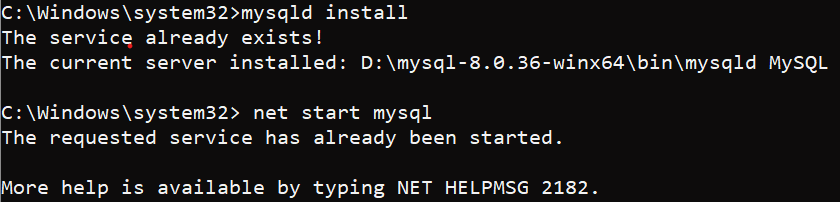
\includegraphics[height=3cm,width=14cm]{1.png}
	\end{figure}
\section{任务一}
根据所给 Student.csv、 Teacher.csv、 Course.csv、 Score.csv 表中的数据信息,在数
据库中创建对应的关系表并将数据录入到数据库中。
\begin{lstlisting}[language=sql]
create schema s_t_c_s;  
create table student(
	SNO char(11) primary key,  
	NAME varchar(4),  
	GENDER varchar(6),  
	BIRTHDAY datetime,  
	DEPART int  
);  
  
insert into student (SNO, NAME, GENDER, BIRTHDAY, DEPART)  
values
('PB210000001', 'YH', 'male', '2002-03-29 00:00:00', 229),
('PB210000002', 'ZY', 'male', '2001-09-12 00:00:00', 11),
('PB210000003', 'FWJ', 'male', '2001-04-29 00:00:00', 12),
('PB210000004', 'JTY', 'male', '2002-03-15 00:00:00', 11),
('PB210000005', 'YY', 'female', '2002-08-12 00:00:00', 12),
('PB210000006', 'HCC', 'male', '2002-06-25 00:00:00', 229),
('PB210000007', 'RZJ', 'male', '2002-06-14 00:00:00', 11),
('PB210000008', 'WCS', 'male', '2002-08-23 00:00:00', 13),
('PB210000009', 'ZMS', 'female', '2002-06-23 00:00:00', 12),
('PB210000010', 'WD', 'male', '2003-02-24 00:00:00', 13),
('PB210000011', 'BL', 'female', '2002-05-08 00:00:00', 14),
('PB210000012', 'ADN', 'male', '2004-06-26 00:00:00', 10),
('PB210000013', 'HD', 'male', '2003-11-17 00:00:00', 14),
('PB210000014', 'GNJ', 'male', '2001-01-28 00:00:00', 11),
('PB210000015', 'XB', 'female', '2002-10-09 00:00:00', 12),
('PB210000016', 'LC', 'female', '2003-11-30 00:00:00', 11),
('PB210000017', 'TX', 'male', '2002-05-16 00:00:00', 12),
('PB210000018', 'MY', 'male', '2003-12-02 00:00:00', 14),
('PB210000019', 'MT', 'female', '2002-02-13 00:00:00', 10),
('PB210000020', 'XY', 'female', '2001-02-14 00:00:00', 229),
('PB210000021', 'LYH', 'male', '2002-09-30 00:00:00', 229),
('PB210000022', 'MSW', 'male', '2003-06-17 00:00:00', 11),
('PB210000023', 'HXY', 'male', '2003-02-18 00:00:00', 12),
('PB210000024', 'YHS', 'female', '2003-04-01 00:00:00', 229),
('PB210000025', 'YWB', 'male', '2003-08-12 00:00:00', 229);

create table teacher(
	TNO char(7) primary key,  
	NAME varchar(4),  
    GENDER varchar(6),  
    BIRTHDAY datetime,  
    POSITION varchar(30),  
    DEPART int  
);  
  
insert into teacher (TNO, NAME, GENDER, BIRTHDAY, POSITION, DEPART)  
values
('TA90021', 'HMZ', 'male', '1994/12/23 00:00:00', 'Instructor', 11),
('TA90022', 'HB', 'female', '1978/4/9 00:00:00', 'Associate Professor', 10),
('TA90023', 'ZDH', 'male', '1986/11/17 00:00:00', 'Instructor', 229),
('TA90024', 'HS', 'male', '1977/4/10 00:00:00', 'Associate Professor', 6),
('TA90025', 'HTZ', 'female', '1969/7/28 00:00:00', 'Professor', 11),
('TA90026', 'TJY', 'male', '1973/10/3 00:00:00', 'Associate Professor', 12),
('TA90027', 'XR', 'male', '1970/5/16 00:00:00', 'Associate Professor', 11),
('TA90028', 'ZXY', 'male', '1986/7/16 00:00:00', 'Instructor', 229),
('TA90029', 'ZR', 'male', '1975/9/24 00:00:00', 'Associate Professor', 11),
('TA90030', 'SY', 'male', '1972/11/6 00:00:00', 'Professor', 229),
('TA90031', 'LQA', 'female', '1986/11/17 00:00:00', 'Associate Professor', 10),
('TA90032', 'GHJ', 'male', '1976/10/1 00:00:00', 'Associate Professor', 18);

create table course(
	CNO char(8) primary key,   
	NAME varchar(50),   
	TYPE int,   
	TNO char(7),  
	foreign key(TNO) references teacher(TNO)  
);  
    
insert into course (CNO, NAME, TYPE, TNO)
values
('20230400', 'Linear_Algebra', '1', 'TA90022'),
('20230402', 'DB_Design', '1', 'TA90021'),
('20230404', 'Machine_Learning', '1', 'TA90023'),
('20230406', 'Operating_System', '1', 'TA90025'),
('20230408', 'Natural_Language_Processing', '0', 'TA90027'),
('20230410', 'Artificial_Intelligence', '1', 'TA90025'),
('20230412', 'Data_Mining', '1', 'TA90025'),
('20230414', 'Signal_Control', '1', 'TA90024'),
('20230416', 'Computer_Network', '1', 'TA90029'),
('20230418', 'Pattern_Recognition', '1', 'TA90023'),
('20230420', 'Deep_Learning', '0', 'TA90030');

create table score (  
    SNO char(11),  
    CNO char(8),  
    DEGREE int,  
    primary key (SNO, CNO),  
    foreign key (SNO) references student(SNO),  
    foreign key (CNO) references course(CNO)  
);


insert into score (SNO, CNO, DEGREE)
values
('PB210000001', '20230402', 89),
('PB210000002', '20230402', 94),
('PB210000003', '20230402', 90),
('PB210000004', '20230402', 95),
('PB210000005', '20230402', 93),
('PB210000006', '20230402', 75),
('PB210000007', '20230402', 78),
('PB210000008', '20230402', 81),
('PB210000001', '20230404', 73),
('PB210000002', '20230404', 82),
('PB210000003', '20230404', 92),
('PB210000004', '20230404', 68),
('PB210000005', '20230404', 72),
('PB210000006', '20230404', 93),
('PB210000007', '20230400', 77),
('PB210000008', '20230400', 92),
('PB210000009', '20230400', 82),
('PB210000010', '20230400', 91),
('PB210000008', '20230418', 69),
('PB210000001', '20230418', 92),
('PB210000002', '20230418', 95),
('PB210000003', '20230418', 82),
('PB210000010', '20230406', 83),
('PB210000011', '20230406', 84),
('PB210000012', '20230406', 78),
('PB210000013', '20230406', 89),
('PB210000017', '20230408', 81),
('PB210000015', '20230408', 74),
('PB210000018', '20230408', 95),
('PB210000019', '20230408', 91),
('PB210000020', '20230408', 89),
('PB210000014', '20230410', 82),
('PB210000016', '20230410', 72),
('PB210000011', '20230410', 75),
('PB210000018', '20230412', 85),
('PB210000020', '20230412', 83),
('PB210000008', '20230412', 77),
('PB210000005', '20230412', 74),
('PB210000015', '20230412', 98),
('PB210000001', '20230412', 80),
('PB210000019', '20230412', 81),
('PB210000019', '20230416', 75),
('PB210000020', '20230416', 89),
('PB210000001', '20230416', 49),
('PB210000002', '20230416', 87),
('PB210000003', '20230416', 97),
('PB210000004', '20230416', 86),
('PB210000005', '20230416', 89),
('PB210000006', '20230418', 90),
('PB210000020', '20230418', 85),
('PB210000021', '20230418', 83),
('PB210000001', '20230420', 95),
('PB210000006', '20230420', 89),
('PB210000020', '20230420', 85),
('PB210000021', '20230420', 83),
('PB210000024', '20230420', 80),
('PB210000025', '20230420', 87);

select * from student;  
select * from teacher;  
select * from course;  
select * from score;  
	\end{lstlisting}
	\begin{figure}[H]
		\centering 
		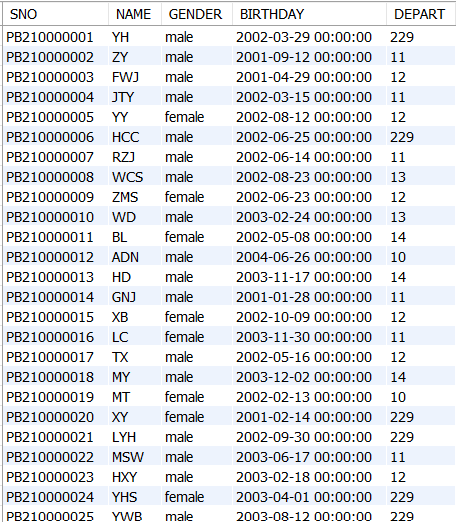
\includegraphics[height=8cm,width=6cm]{2.png}
		\end{figure}
		\begin{figure}[H]
			\centering 
			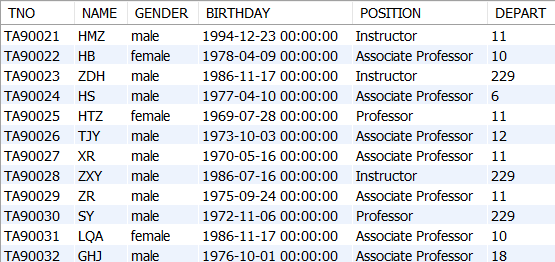
\includegraphics[height=3.5cm,width=6cm]{3.png}
			\end{figure}
			\begin{figure}[H]
				\centering 
				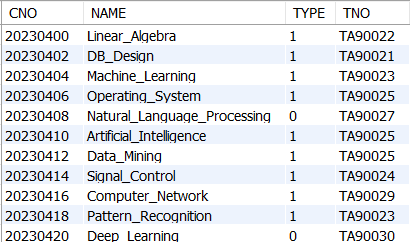
\includegraphics[height=3cm,width=6cm]{4.png}
				\end{figure}
				\begin{figure}[H]
					\centering 
					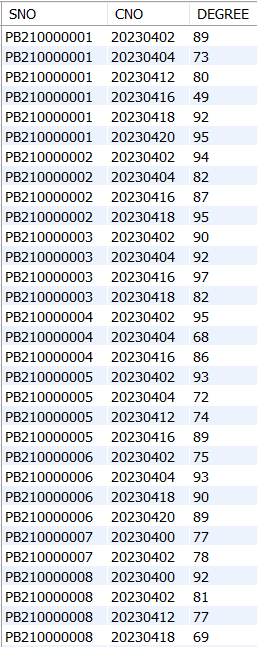
\includegraphics[height=12cm,width=6cm]{5.png}
					\end{figure}
					\begin{figure}[H]
						\centering 
						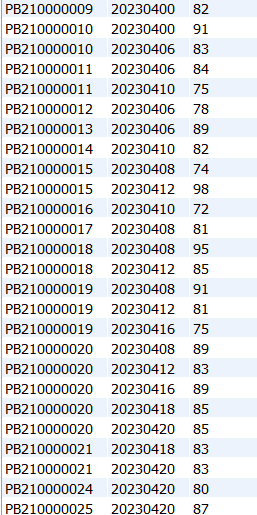
\includegraphics[height=9cm,width=6cm]{6.png}
						\end{figure}
\section{任务二:实现以下各题功能的 SQL 语句}

\subsection{修改基本表}
\subsubsection{在学生表 student 中增加一个新的属性列 AGE(年龄),类型为 int}
\begin{lstlisting}[language=sql]
	alter table student add AGE int;  
\end{lstlisting}
\subsubsection{计算每个学生的年龄(AGE)}
\begin{lstlisting}[language=sql]
set sql_safe_updates = 0;  
update student set AGE = YEAR(CURDATE()) - YEAR(BIRTHDAY);  
select AGE from student;  
\end{lstlisting}
\begin{figure}[H]
	\centering 
	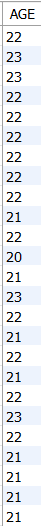
\includegraphics[height=7cm,width=14cm]{7.png}
	\end{figure}
\subsubsection{为每个学生的年龄加2, 将 AGE的数据类型由int改为char}
\begin{lstlisting}[language=sql]
	update student set AGE = AGE + 2;  
	select AGE from student;  
	  
	alter table student modify column AGE CHAR(2);
\end{lstlisting}
\begin{figure}[H]
	\centering 
	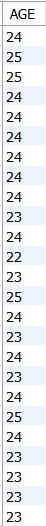
\includegraphics[height=7cm,width=14cm]{8.png}
	\end{figure}
	\begin{figure}[H]
		\centering 
		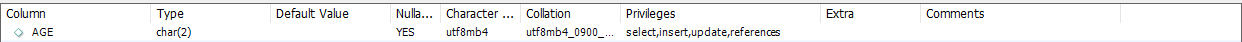
\includegraphics[height=7cm,width=14cm]{9.png}
		\end{figure}
\subsubsection{删除属性列 AGE}
\begin{lstlisting}[language=sql]
alter table student drop column AGE;  
select * from student;
\end{lstlisting}
\begin{figure}[H]
	\centering 
	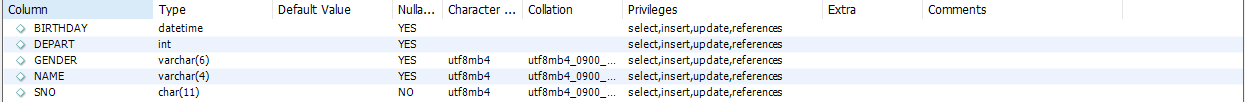
\includegraphics[height=7cm,width=14cm]{10.png}
	\end{figure}
\subsubsection{创建一个教师课程数量表:teacher\_course(TNO,NUM\_COURSE),两个属性分别表示授课教师工号,课程数量,其中TNO是主键}
\begin{lstlisting}[language=sql]
	
\end{lstlisting}
\begin{figure}[H]
	\centering 
	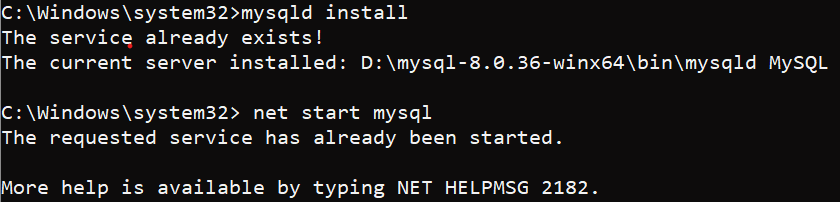
\includegraphics[height=7cm,width=14cm]{1.png}
	\end{figure}
\subsubsection{用一条语句,结合表 course 记录,为表 teacher 中所有教师,在表 teacher\_course 添加对应记录(若表 course 中未出现的教师,则课程数量记为 NULL)}
\begin{lstlisting}[language=sql]
	
\end{lstlisting}
\begin{figure}[H]
	\centering 
	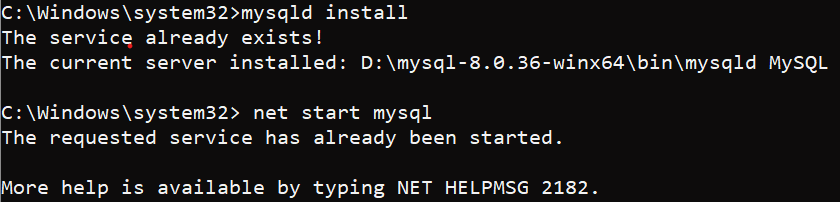
\includegraphics[height=7cm,width=14cm]{1.png}
	\end{figure}
\subsubsection{删除表 teacher\_course 中含有 NULL 的记录}\begin{lstlisting}[language=sql]
	
\end{lstlisting}
\begin{figure}[H]
	\centering 
	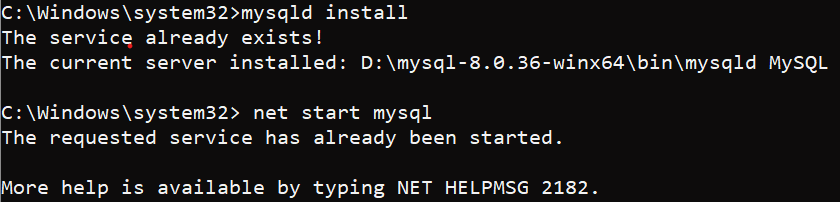
\includegraphics[height=7cm,width=14cm]{1.png}
	\end{figure}
\subsubsection{删除表 teacher\_course}
\begin{lstlisting}[language=sql]
	
\end{lstlisting}
\begin{figure}[H]
	\centering 
	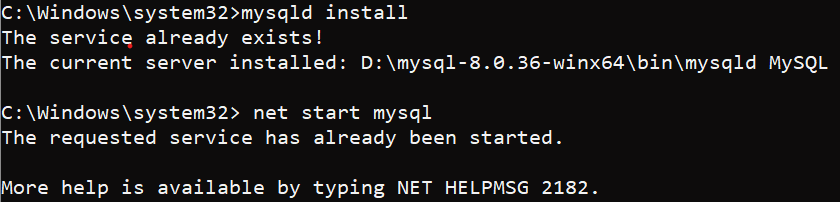
\includegraphics[height=7cm,width=14cm]{1.png}
	\end{figure}
\subsubsection{在学生表 student 、成绩表 score 中分别插入一些数据}
\begin{lstlisting}[language=sql]
	
\end{lstlisting}
\begin{figure}[H]
	\centering 
	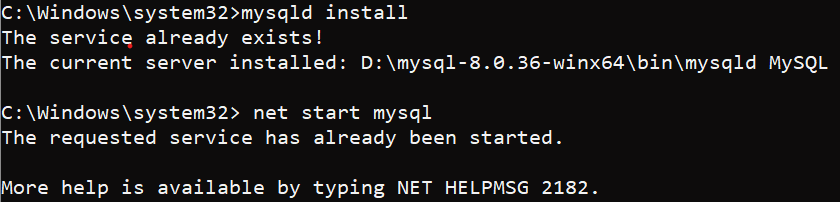
\includegraphics[height=7cm,width=14cm]{1.png}
	\end{figure}
\subsubsection{在 score 表中删除你所选的课程中成绩最低的一门课程的记录(可能会用到子查询)}
\begin{lstlisting}[language=sql]
	
\end{lstlisting}
\begin{figure}[H]
	\centering 
	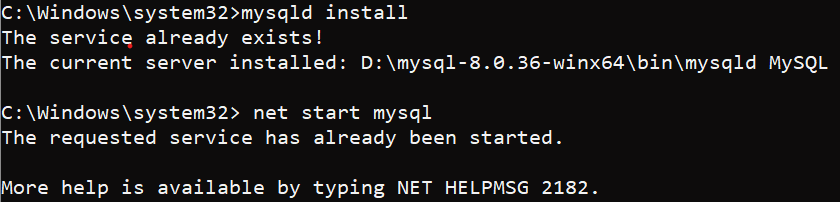
\includegraphics[height=7cm,width=14cm]{1.png}
	\end{figure}
\subsection{索引}
\subsubsection{用 create 语句在 course 表的名称 NAME 上建立普通索引 NAME\_INDEX}
\begin{lstlisting}[language=sql]
	
\end{lstlisting}
\begin{figure}[H]
	\centering 
	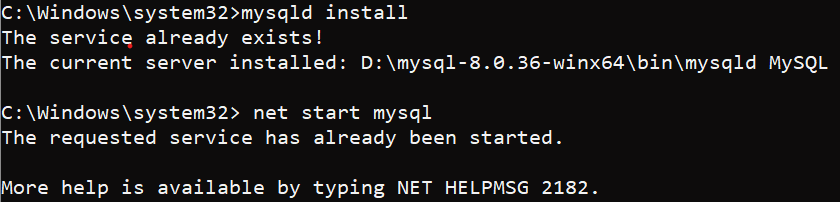
\includegraphics[height=7cm,width=14cm]{1.png}
	\end{figure}
\subsubsection{用 create 语句在 teacher 表的工号 TNO 上建立唯一索引 TNO\_INDEX}
\begin{lstlisting}[language=sql]
	
\end{lstlisting}
\begin{figure}[H]
	\centering 
	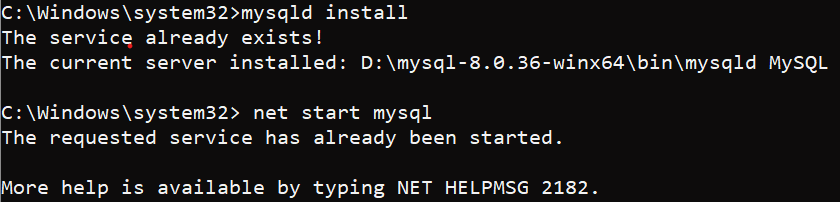
\includegraphics[height=7cm,width=14cm]{1.png}
	\end{figure}
\subsubsection{用 create 语 句 在 score 表 上 的 学 号 SNO 、 成 绩 DEGREE 上 建 立 复 合 索引RECORD\_INDEX, 要求学号为降序,学号相同时成绩为升序}
\begin{lstlisting}[language=sql]
	
\end{lstlisting}
\begin{figure}[H]
	\centering 
	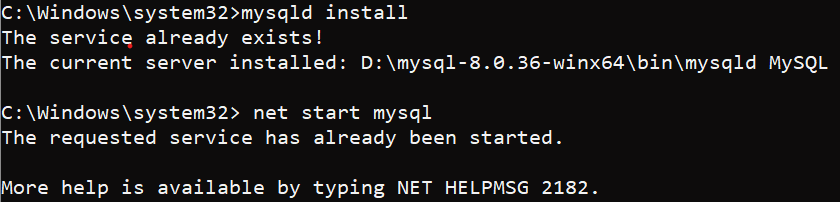
\includegraphics[height=7cm,width=14cm]{1.png}
	\end{figure}
\subsubsection{用一条语句查询表 score 的索引}
\begin{lstlisting}[language=sql]
	
\end{lstlisting}
\begin{figure}[H]
	\centering 
	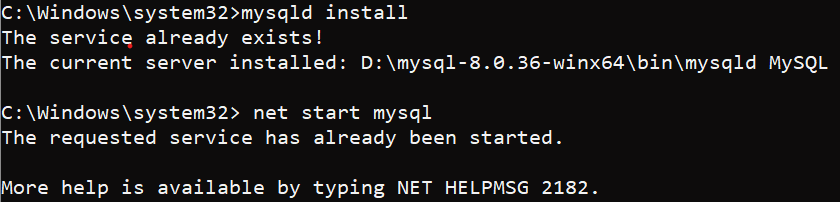
\includegraphics[height=7cm,width=14cm]{1.png}
	\end{figure}
\subsubsection{删除 teacher 表字段 TNO 上的索引 TNO\_INDEX}
\begin{lstlisting}[language=sql]
	
\end{lstlisting}
\begin{figure}[H]
	\centering 
	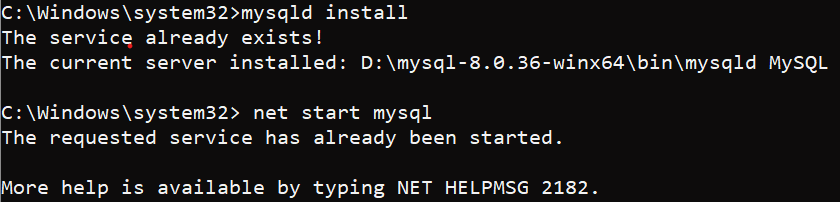
\includegraphics[height=7cm,width=14cm]{1.png}
	\end{figure}
\subsection{查询}
\subsubsection{查询和你属于同一个系的学生学号和姓名(包括你本人)}
\begin{lstlisting}[language=sql]
	
\end{lstlisting}
\begin{figure}[H]
	\centering 
	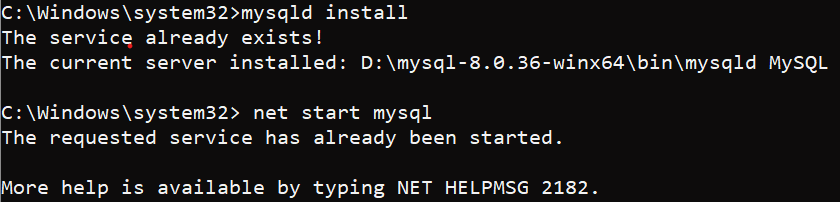
\includegraphics[height=7cm,width=14cm]{1.png}
	\end{figure}
\subsubsection{查询和你属于同一个系的学生学号和姓名(不包括你本人)}
\begin{lstlisting}[language=sql]
	
\end{lstlisting}
\begin{figure}[H]
	\centering 
	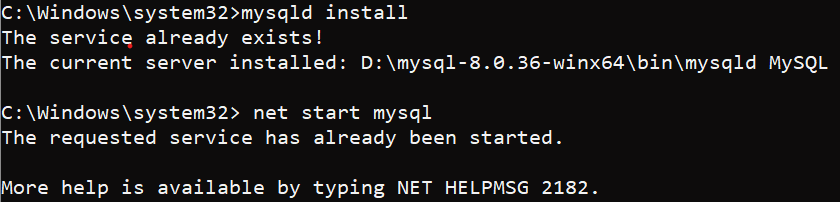
\includegraphics[height=7cm,width=14cm]{1.png}
	\end{figure}
\subsubsection{查询和你的某个好友属于同一个系的学生学号和姓名(9 题插入的某个好友)}
\begin{lstlisting}[language=sql]
	
\end{lstlisting}
\begin{figure}[H]
	\centering 
	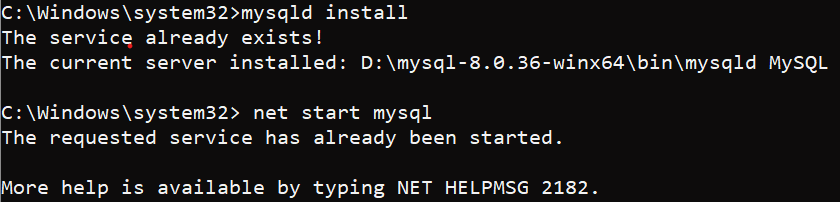
\includegraphics[height=7cm,width=14cm]{1.png}
	\end{figure}
\subsubsection{查询和你的两个好友都不在一个系的学生学号和姓名(9 题插入的两个好友)}
\begin{lstlisting}[language=sql]
	
\end{lstlisting}
\begin{figure}[H]
	\centering 
	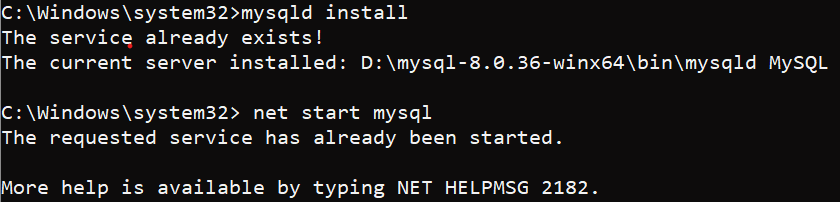
\includegraphics[height=7cm,width=14cm]{1.png}
	\end{figure}
\subsubsection{查询教过你的所有老师的工号和姓名}
\begin{lstlisting}[language=sql]
	
\end{lstlisting}
\begin{figure}[H]
	\centering 
	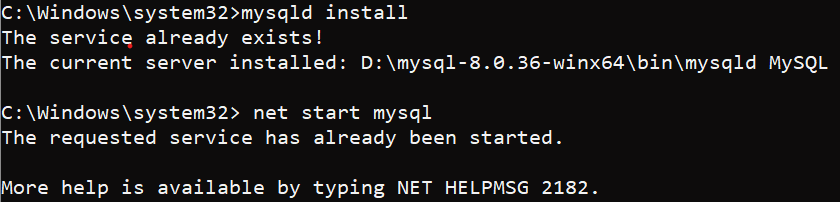
\includegraphics[height=7cm,width=14cm]{1.png}
	\end{figure}
\subsubsection{查询 11 系和 229 系教师的总人数}
\begin{lstlisting}[language=sql]
	
\end{lstlisting}
\begin{figure}[H]
	\centering 
	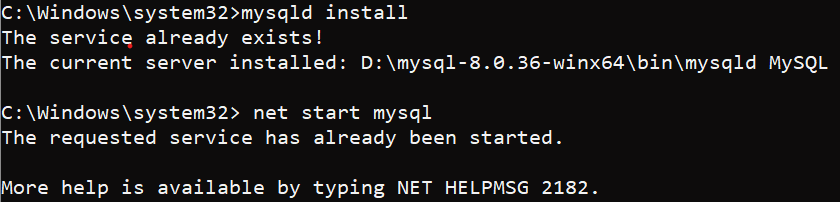
\includegraphics[height=7cm,width=14cm]{1.png}
	\end{figure}
\subsubsection{查询你的系中年龄(即当前年份减去出生年份) 最大的学生的学号、姓名和年龄}
\begin{lstlisting}[language=sql]
	
\end{lstlisting}
\begin{figure}[H]
	\centering 
	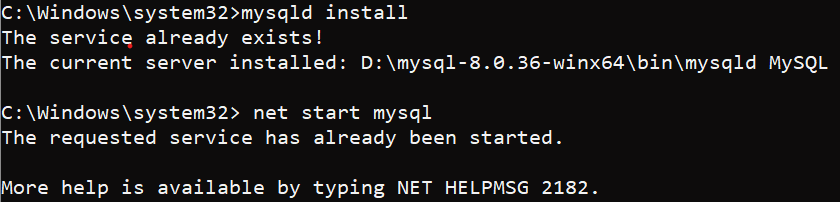
\includegraphics[height=7cm,width=14cm]{1.png}
	\end{figure}
\subsubsection{查询你的系中年龄(即当前年份减去出生年份) 最小的学生的学号、姓名和年龄}
\begin{lstlisting}[language=sql]
	
\end{lstlisting}
\begin{figure}[H]
	\centering 
	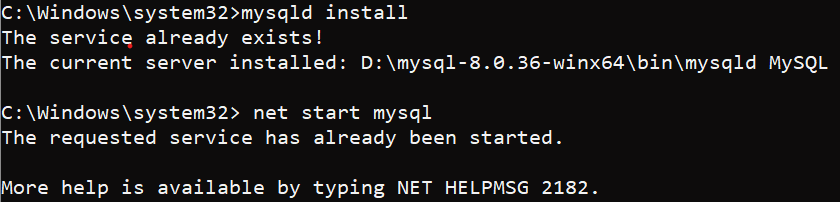
\includegraphics[height=7cm,width=14cm]{1.png}
	\end{figure}
\subsubsection{查询选修 DB\_Design 课程且成绩在 75 分以下(不包括 75) 的学生的学号、姓名和分数}
\begin{lstlisting}[language=sql]
	
\end{lstlisting}
\begin{figure}[H]
	\centering 
	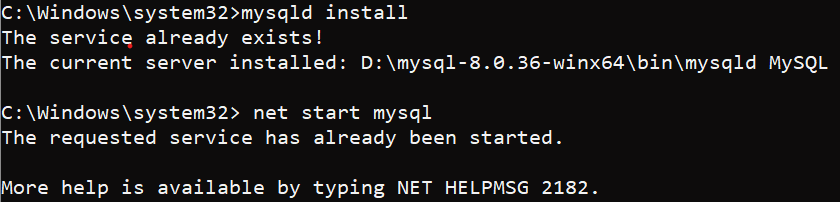
\includegraphics[height=7cm,width=14cm]{1.png}
	\end{figure}
\subsubsection{查询选修过“ZDH”老师课程的学生学号和姓名(去掉重复行)}
\begin{lstlisting}[language=sql]
	
\end{lstlisting}
\begin{figure}[H]
	\centering 
	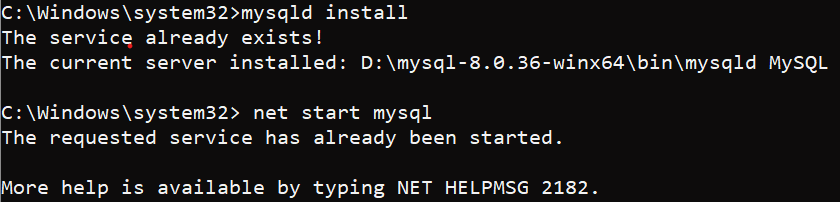
\includegraphics[height=7cm,width=14cm]{1.png}
	\end{figure}
\subsubsection{查询选过某课程的学生学号和分数,并按分数降序展示}
\begin{lstlisting}[language=sql]
	
\end{lstlisting}
\begin{figure}[H]
	\centering 
	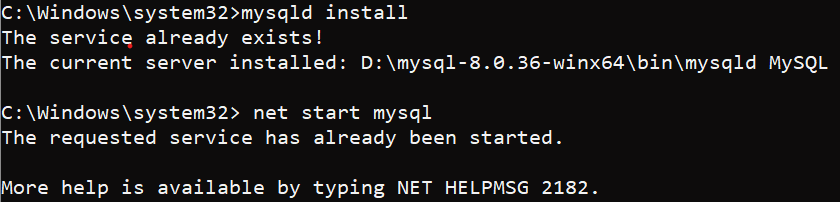
\includegraphics[height=7cm,width=14cm]{1.png}
	\end{figure}
\subsubsection{查询每门课的平均成绩,其中每行包含课程号、课程名和平均成绩(包括平均成绩为NULL,即该课没有成绩)}
\begin{lstlisting}[language=sql]
	
\end{lstlisting}
\begin{figure}[H]
	\centering 
	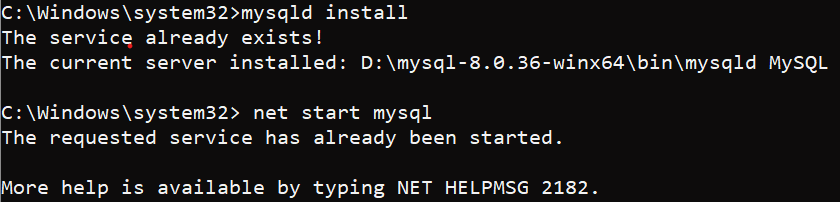
\includegraphics[height=7cm,width=14cm]{1.png}
	\end{figure}
\subsubsection{查询每门必修课的平均成绩,其中每行包含课程号、课程名和平均成绩(包括平均成绩为NULL,即该课没有成绩)}
\begin{lstlisting}[language=sql]
	
\end{lstlisting}
\begin{figure}[H]
	\centering 
	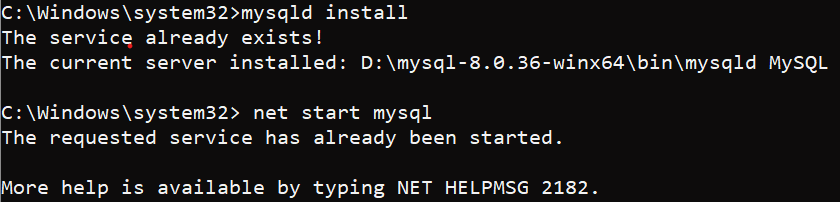
\includegraphics[height=7cm,width=14cm]{1.png}
	\end{figure}
\subsubsection{查询至少选修了 ZDH 老师(TNO=”TA90023”)开设的所有课程的学生学号}
\begin{lstlisting}[language=sql]
	
\end{lstlisting}
\begin{figure}[H]
	\centering 
	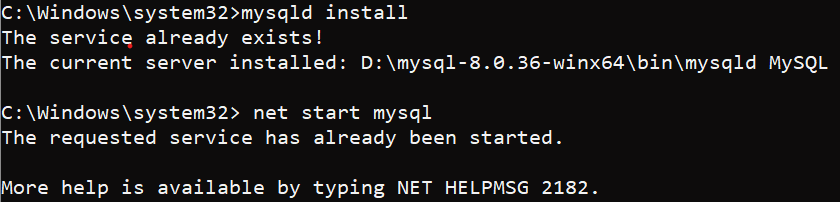
\includegraphics[height=7cm,width=14cm]{1.png}
	\end{figure}
\subsubsection{查询每门课程的最高分和最低分,并计算其分数差。其中每行包含课程号、课程名和最高分、最低分和分数差(课程无成绩的不用包括)}
\begin{lstlisting}[language=sql]
	
\end{lstlisting}
\begin{figure}[H]
	\centering 
	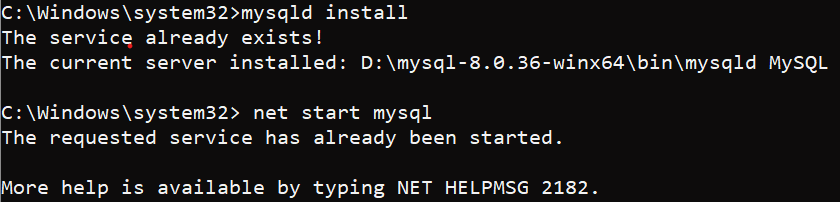
\includegraphics[height=7cm,width=14cm]{1.png}
	\end{figure}
\subsubsection{查询存在考试成绩低于 75 分的学生学号,以及低于 75 分的课程数量}
\begin{lstlisting}[language=sql]
	
\end{lstlisting}
\begin{figure}[H]
	\centering 
	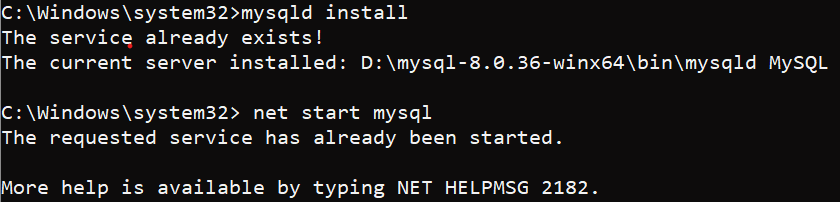
\includegraphics[height=7cm,width=14cm]{1.png}
	\end{figure}
\subsubsection{查询所教过的课程中有学生考试成绩低于 75 分的教师的工号和姓名(去掉重复行)}
\begin{lstlisting}[language=sql]
	
\end{lstlisting}
\begin{figure}[H]
	\centering 
	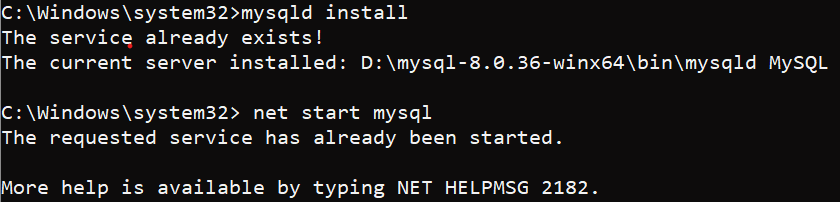
\includegraphics[height=7cm,width=14cm]{1.png}
	\end{figure}
\subsubsection{查询选修少于 2 门课程的学生的学号、姓名}
\begin{lstlisting}[language=sql]
	
\end{lstlisting}
\begin{figure}[H]
	\centering 
	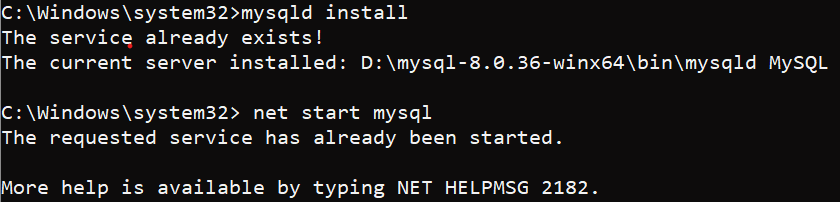
\includegraphics[height=7cm,width=14cm]{1.png}
	\end{figure}
\subsubsection{查询至少选修了 YH 同学(SNO=”PB210000001”)所选全部课程的学生学号}
\begin{lstlisting}[language=sql]
	
\end{lstlisting}
\begin{figure}[H]
	\centering 
	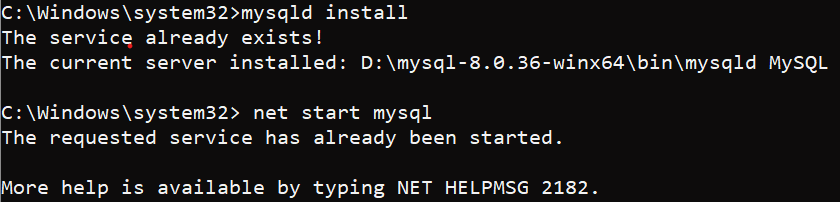
\includegraphics[height=7cm,width=14cm]{1.png}
	\end{figure}
\subsubsection{查询 Course 表中各个课程名称与相应的平均成绩(没有选课的学生平均成绩为 NULL) }
\begin{lstlisting}[language=sql]
	
\end{lstlisting}
\begin{figure}[H]
	\centering 
	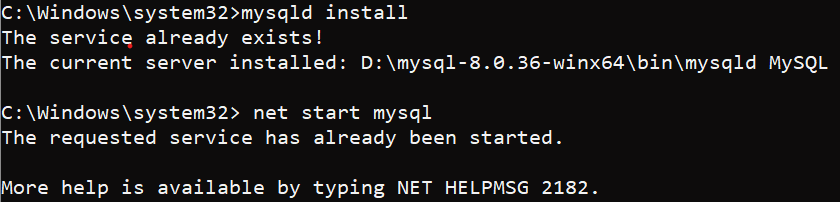
\includegraphics[height=7cm,width=14cm]{1.png}
	\end{figure}
\subsubsection{查询每个系的学生人数和每个系的平均分,其中每行包含系号、系的人数和平均成绩}
\begin{lstlisting}[language=sql]
	
\end{lstlisting}
\begin{figure}[H]
	\centering 
	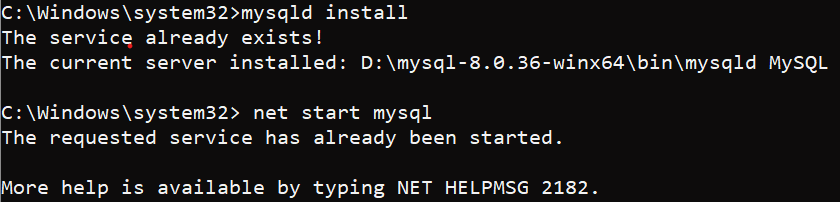
\includegraphics[height=7cm,width=14cm]{1.png}
	\end{figure}
\subsubsection{查询所有未选修 DB\_Design 课程或者 Data\_Mining 课程的学生的学生姓名(去掉重复行)}
\begin{lstlisting}[language=sql]
	
\end{lstlisting}
\begin{figure}[H]
	\centering 
	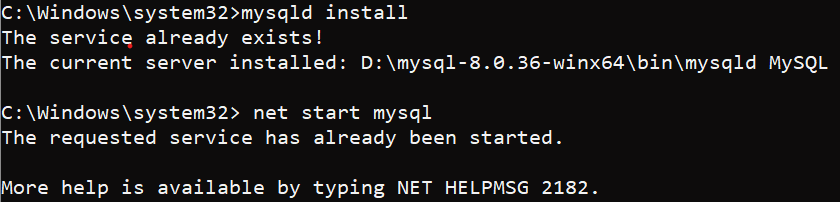
\includegraphics[height=7cm,width=14cm]{1.png}
	\end{figure}
\subsubsection{查询各个课程的课程名及选该课的学生的最小年龄、最大年龄和平均年龄。(包括没有人选的课)}
\begin{lstlisting}[language=sql]
	
\end{lstlisting}
\begin{figure}[H]
	\centering 
	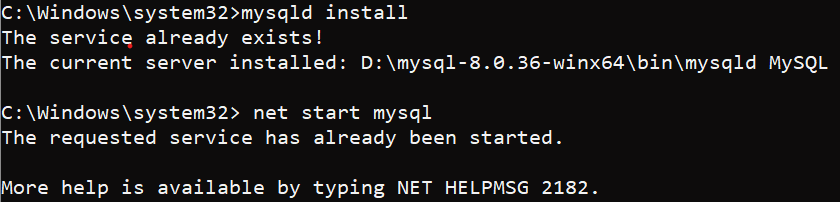
\includegraphics[height=7cm,width=14cm]{1.png}
	\end{figure}
\subsubsection{查询选修了课程名中包含”Computer”课程的学生的学号和姓名}
\begin{lstlisting}[language=sql]
	
\end{lstlisting}
\begin{figure}[H]
	\centering 
	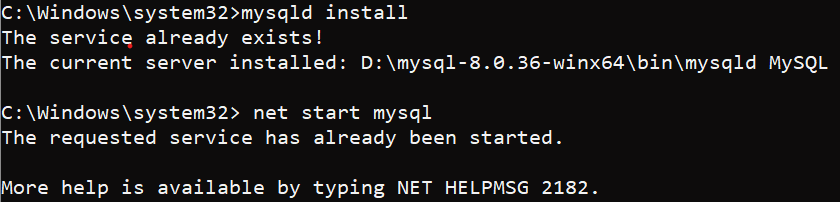
\includegraphics[height=7cm,width=14cm]{1.png}
	\end{figure}
\subsubsection{设课程平均成绩为 x,查询各个课程成绩处于[x-12, x+12]区间的同学的成绩表,即包含 SNO、CNO、 DEGREE}
\begin{lstlisting}[language=sql]
	
\end{lstlisting}
\begin{figure}[H]
	\centering 
	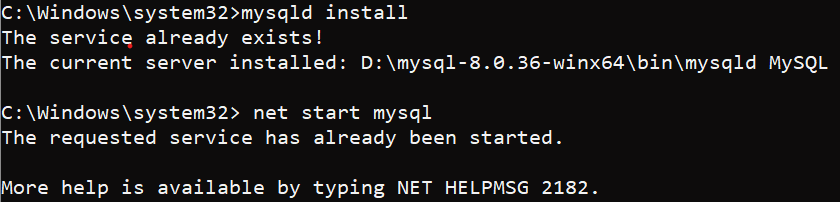
\includegraphics[height=7cm,width=14cm]{1.png}
	\end{figure}
\subsection{视图}
\subsubsection{建立 229 系的学生视图(db\_22\_student),属性与 student 表一样,并要求对该视图进行修改和插入操作时仍需保证该视图只有 229 系的学生}
\begin{lstlisting}[language=sql]
	
\end{lstlisting}
\begin{figure}[H]
	\centering 
	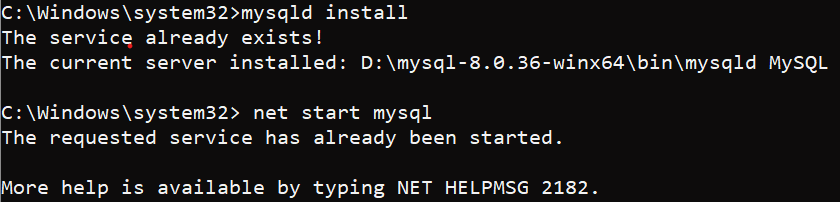
\includegraphics[height=7cm,width=14cm]{1.png}
	\end{figure}
\subsubsection{将 229 系学生视图(db\_229\_student)中学号为“PB210000020”的学生姓名改为{你的姓名(英文首字母)}}
\begin{lstlisting}[language=sql]
	
\end{lstlisting}
\begin{figure}[H]
	\centering 
	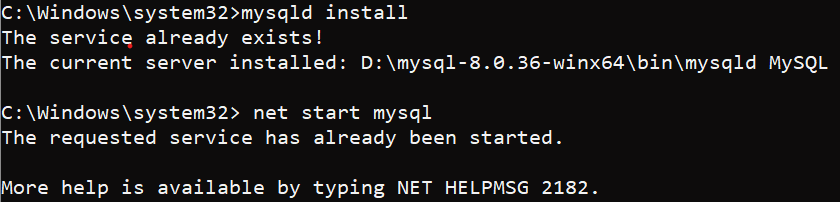
\includegraphics[height=7cm,width=14cm]{1.png}
	\end{figure}
\subsubsection{在 229 系学生视图(db\_229\_student)中找出年龄小于 22 岁的学生,包含 SNO、 NAME}
\begin{lstlisting}[language=sql]
	
\end{lstlisting}
\begin{figure}[H]
	\centering 
	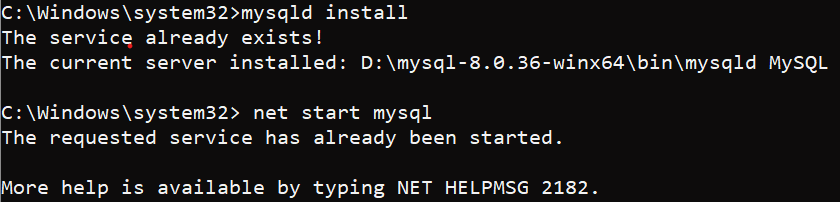
\includegraphics[height=7cm,width=14cm]{1.png}
	\end{figure}
\subsubsection{向 student 表中插入一名“学号 SA210110021,姓名 QXY,性别女,生日 2007/7/27, 229系”的学生。然后查询视图 db\_229\_student 的所有学生,验证其是否更新}
\begin{lstlisting}[language=sql]
	
\end{lstlisting}
\begin{figure}[H]
	\centering 
	\includegraphics[height=7cm,width=14cm]{1.png}
	\end{figure}
\subsubsection{向视图 db\_229\_student 中插入一名“学号 SA210110023,姓名 DPC,性别男,生日1997/4/27, 11 系”的学生,观察到了什么现象?}
\begin{lstlisting}[language=sql]
	
\end{lstlisting}
\begin{figure}[H]
	\centering 
	\includegraphics[height=7cm,width=14cm]{1.png}
	\end{figure}
\subsubsection{删除视图 db\_229\_student}
\begin{lstlisting}[language=sql]
	drop view db_229_student;
\end{lstlisting}
\subsection{触发器}
\subsubsection{创建关系表: teacher\_salary(TNO, SAL),其中 TNO 是教师工号(主键), SAL 是教师工资(类型 float)}
\begin{lstlisting}[language=sql]
	
\end{lstlisting}
\begin{figure}[H]
	\centering 
	\includegraphics[height=7cm,width=14cm]{1.png}
	\end{figure}
\subsubsection{定义一个 BEFORE 行级触发器,为关系表 teacher\_salary 定义完整性规则: “表中出现的工号必须也出现在 teacher 表中,否则报错”。}

\begin{lstlisting}[language=sql]
	
\end{lstlisting}
\begin{figure}[H]
	\centering 
	\includegraphics[height=7cm,width=14cm]{1.png}
	\end{figure}
\subsubsection{定义一个 BEFORE 行级触发器,为关系表 teacher\_salary 定 义 完 整 性 规 则 :
“Instructor/Associate Professor/Professor 的工资不能低于 4000/7000/10000,且不能高于
7000/10000/13000,如果低于,则改为 4000/7000/10000”,如果高于,则改为 7000/10000/13000}
\begin{lstlisting}[language=sql]
	
\end{lstlisting}
\begin{figure}[H]
	\centering 
	\includegraphics[height=7cm,width=14cm]{1.png}
	\end{figure}
\subsubsection{删除刚刚创建的所有触发器}
\begin{lstlisting}[language=sql]
	
\end{lstlisting}
\begin{figure}[H]
	\centering 
	\includegraphics[height=7cm,width=14cm]{1.png}
	\end{figure}
\subsection{空值}
\subsubsection{将 score 表中的 Data\_Mining 课程成绩设为空值,然后在 score 表查询学生学号和分数,并按分数升序展示。观察 NULL 在 MySQL 中的大小是怎样的}
\begin{lstlisting}[language=sql]
	
\end{lstlisting}
\begin{figure}[H]
	\centering 
	\includegraphics[height=7cm,width=4cm]{58.png}
	\end{figure}
	\begin{figure}[H]
		\centering 
		\includegraphics[height=7cm,width=4cm]{59.png}
		\end{figure}
\subsection{开放题}
\subsubsection{}
\begin{lstlisting}[language=sql]
	
\end{lstlisting}
\begin{figure}[H]
	\centering 
	\includegraphics[height=7cm,width=14cm]{1.png}
	\end{figure}
\subsubsection{}
\begin{lstlisting}[language=sql]
	
\end{lstlisting}
\begin{figure}[H]
	\centering 
	\includegraphics[height=7cm,width=14cm]{1.png}
	\end{figure}
	\section{Conclusion}
    \end{document}